\section{Results \& Evaluation}\label{results}


\subsection{Evaluation Process}

\subsubsection{User Requirements Results}

The user requirements survey was sent out to 11 participants, and the results are shown in Table \ref{table:user-requirements}. The survey was designed to gather information about the participants' experiences with perimenopause and menopause, as well as their preferences for tracking symptoms.

\begin{table}[h!!]
    \caption{User Requirements Survey Results}
    \label{table:user-requirements}
    \resizebox{\textwidth}{!}{
        \begin{tabular}{lll}
        \hline
        User Requirements Survey Results (n = 11)                                       &                        &      \\ \hline
        What stage of menopause are you in?                                             & Premenopausal          & 9\%  \\
                                                                                        & PeriMenopausal         & 55\% \\
                                                                                        & Menopausal             & 0\%  \\
                                                                                        & PostMenopausal         & 18\% \\
                                                                                        & Other                  & 18\% \\
        Do you experience any Period, Perimenopause, or Menopause symptoms?             & Yes                    & 82\% \\
                                                                                        & No                     & 18\% \\
        What peri-menopausal / menopausal symptoms do you currently experience, if any? & Hot Flashes            & 9\%  \\
                                                                                        & Mood Swings            & 13\% \\
                                                                                        & Irregular Periods      & 4\%  \\
                                                                                        & Sleep Problems         & 13\% \\
                                                                                        & Joint and Muscle Aches & 16\% \\
                                                                                        & Vaginal Dryness        & 13\% \\
                                                                                        & Night Sweats           & 6\%  \\
                                                                                        & Have to pee often      & 9\%  \\
                                                                                        & Other                  & 9\%  \\
        How do you track your symptoms or periods?                                      & Smartwatch             & 18\% \\
                                                                                        & Manually recorded      & 36\% \\
                                                                                        & No tracking            & 18\% \\ \hline
        \end{tabular}
    }
  \end{table}

The results show that the majority of participants are in the perimenopausal stage, and most experience symptoms related to this stage. The survey also revealed that many participants do not currently track their symptoms, indicating a potential need for a user-friendly tracking app.

\subsubsection{Round 1: Web App Evaluation}
For the first round of app evaluation, 5 users who were women between the ages of 30 and 65 were recruited to watch a demo video of the app and fill out a SUS and a few long answer questions with their feedback. These participants were recruited via email and were asked to read through a participant information sheet before participating. 

\begin{table}[h!!]
    \caption{Reound 1 SUS Results for Prototype React Web App}
    \label{table:proto-sus}
    \begin{tabular}{ll}
    \hline
    SUS Scores(n=5) &      \\ \hline
                    & 67.5 \\
                    & 85   \\
                    & 72.5 \\
                    & 77.5 \\
                    & 65   \\
        Average Score & 73.5
    \end{tabular}
    \end{table}

Each users sus score was averaged as seen in Figure \ref{table:proto-sus} to produce the average SUS score of 73.5, it is clear that the app is usable as it's in the 27th percentile of app scores, but there is room for improvement. The app got a 3.8 average rating by the 5 users who reviewed this app. Some notes of improvement included:

\begin{itemize}
    \item Inconsistent back buttons
    \item Initial setup could be difficult for some 
    \item Unable to track symptoms hourly
    \item Could use more graphs
    \item The app is not very informative
    \item A page to summaries all symptoms experienced to share with doctor
    \item Text size is too small
    \item Help buttons
\end{itemize}

\subsubsection{Round 2: React Native Evaluation with Group A}

After obtaining these results, changes were made to the app's look and feel and more instructions were included. AB Testing was then conducted with more participants to see if the changes made had a positive impact on the SUS score. 

\begin{table}[]
    \caption{Round 2 SUS Results for Group A React Native App}
    \label{table:grp-a-sus}
    \resizebox{\textwidth}{!}{
    \begin{tabular}{llllllll}
    \hline
    \multicolumn{8}{l}{SUS Group A Results}                                                                                                                \\ \hline
                                                                                            & User 1 & User 2 & User 3 & User 4 & User 5 & User 6 & User 7 \\
    I think that I would like to use PeriPath frequently.                                   & 5      & 5      & 5      & 5      & 5      & 5      & 5      \\
    I found PeriPath unnecessarily complex.                                                 & 1      & 2      & 1      & 2      & 2      & 1      & 1      \\
    I thought PeriPath was easy to use.                                                     & 4      & 5      & 5      & 4      & 4      & 4      & 5      \\
    I think that I would need the support of a technical person to be able to use PeriPath. & 3      & 2      & 3      & 2      & 3      & 3      & 3      \\
    I found the various functions in PeriPath were well integrated.                         & 5      & 4      & 5      & 5      & 4      & 5      & 4      \\
    I thought there was too much inconsistency in PeriPath.                                 & 1      & 1      & 1      & 2      & 2      & 2      & 1      \\
    I would imagine that most people would learn to use PeriPath very quickly.              & 4      & 4      & 5      & 4      & 4      & 4      & 5      \\
    I found PeriPath very cumbersome to use.                                                & 1      & 1      & 1      & 2      & 2      & 2      & 2      \\
    I felt very confident using PeriPath.                                                   & 4      & 4      & 5      & 5      & 5      & 4      & 4      \\
    I needed to learn a lot of things before I could get going with PeriPath.               & 1      & 3      & 1      & 3      & 3      & 3      & 3      \\ \hline
    SUS Score                                                                               & 87.5   & 82.5   & 95     & 80     & 75     & 77.5   & 82.5   \\
    Average SUS Score from all users                                                        & \multicolumn{7}{l}{82.85}                                    \\ \hline
    \end{tabular}
    }
    \end{table}

    From the data in Table \ref{table:grp-a-sus}, the average SUS score was 82.85, which means the app lands in the 82nd percentile. 


    \begin{figure}[h!!]
        \begin{center}
          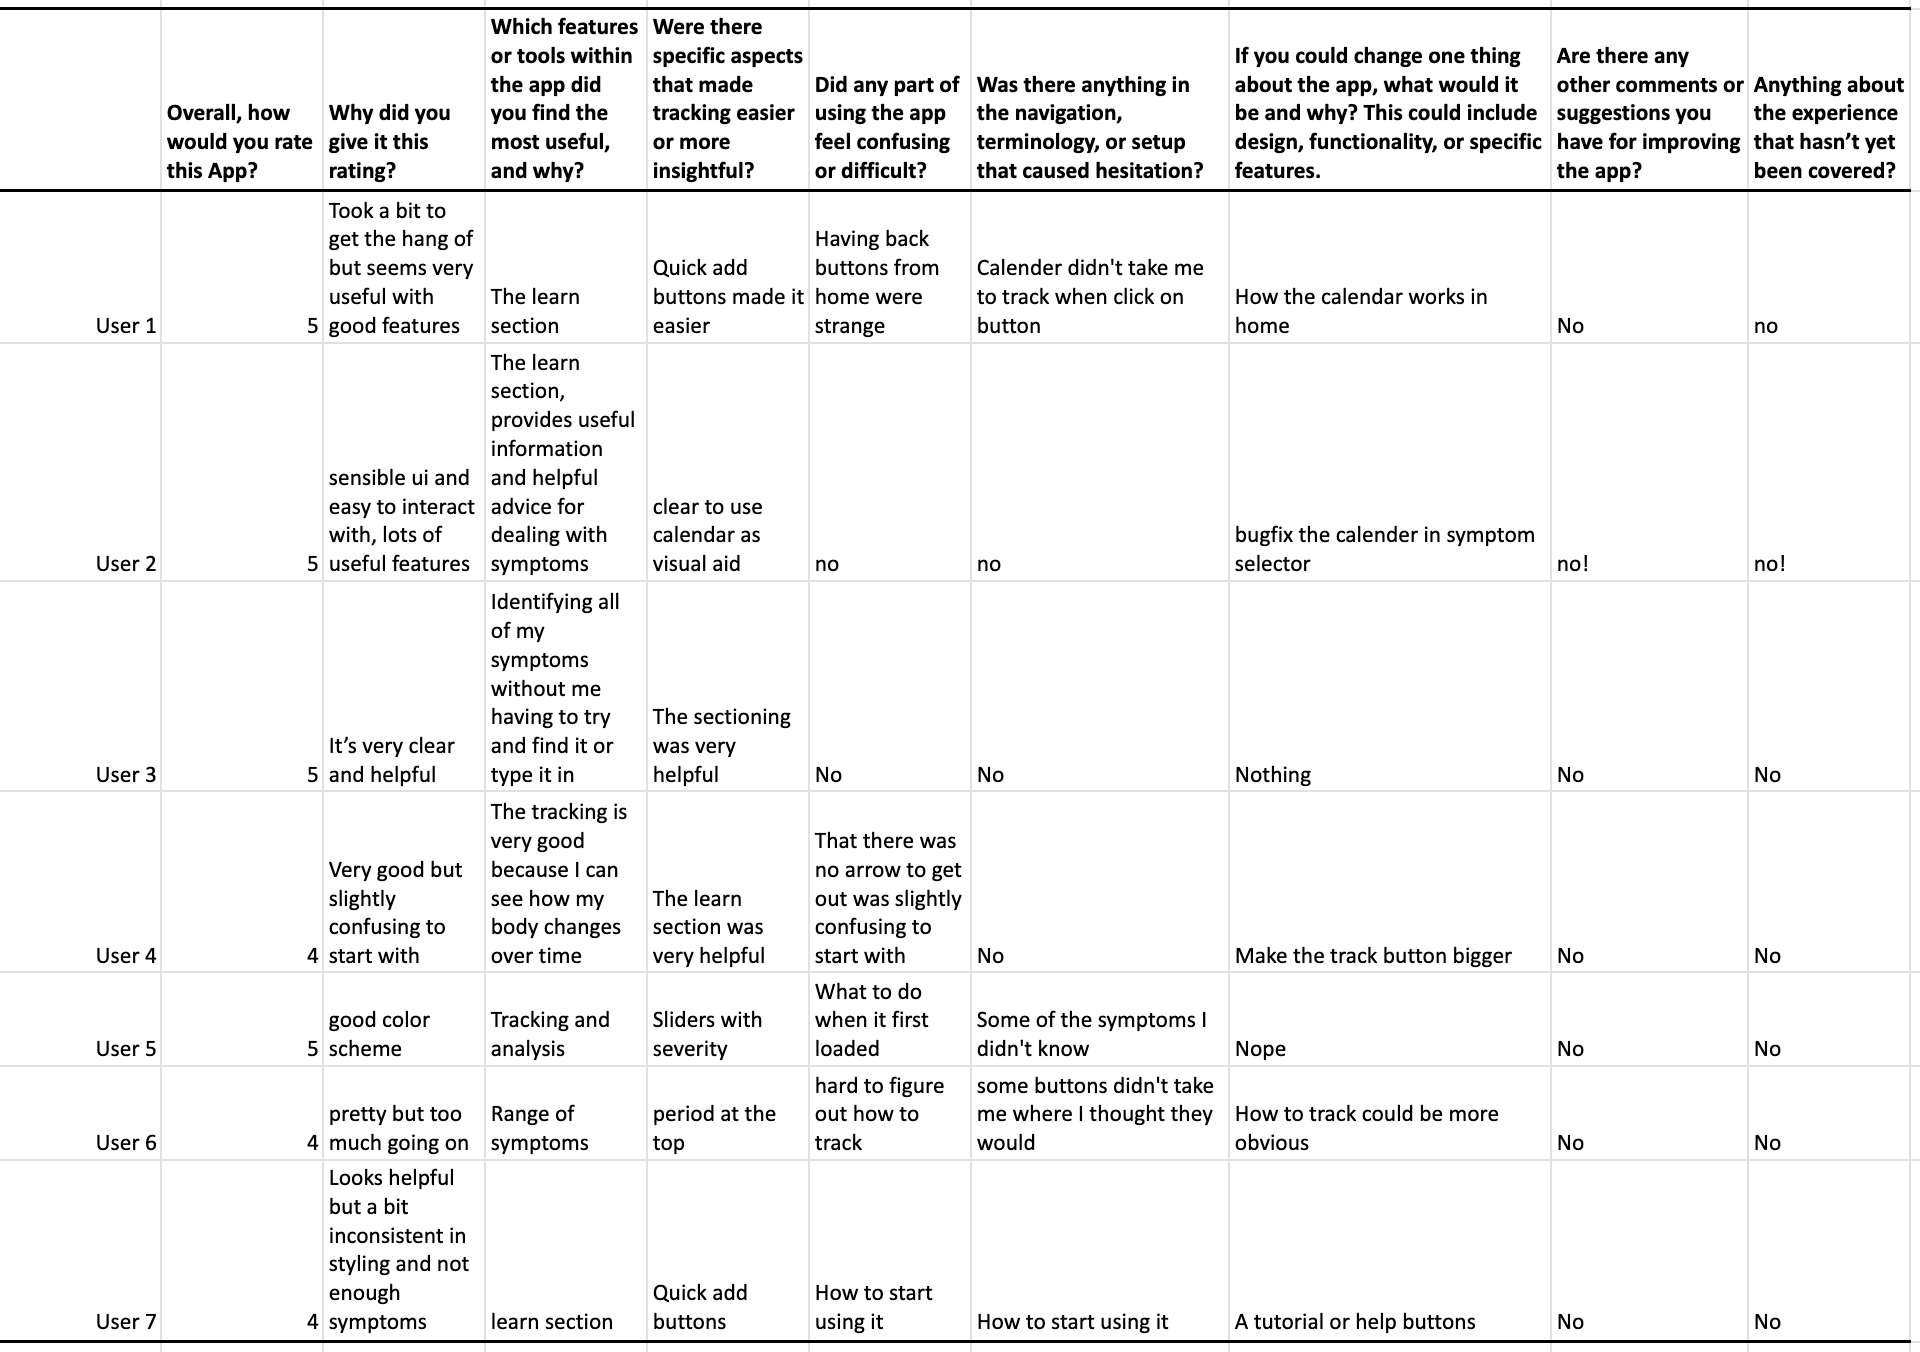
\includegraphics[scale=0.3]{GA-frq.png}
          \caption{Group A Free Response Questions Feedback}
          \label{figure:ga-frq}
        \end{center}
      \end{figure}
    

\subsubsection{Round 3: React Native Evaluation with Group B}
After implementing the feedback from Group A, the app was then tested with a new group of participants. This group was also asked to fill out a SUS and long answer questions about their experience with the app. The goal of this round of testing was to see if the changes made had a positive impact on the usability of the app.

The changes made included: 

\begin{table}[]
    \caption{Round 3 SUS Results for Group B React Native App}
    \label{table:grp-b-sus}
    \resizebox{\textwidth}{!}{
    \begin{tabular}{llllllll}
    \hline
    \multicolumn{8}{l}{SUS Group B Results}                                                                                                                \\ \hline
                                                                                            & User 1 & User 2 & User 3 & User 4 & User 5 & User 6 & User 7 \\
    I think that I would like to use PeriPath frequently.                                   & 5      & 5      & 5      & 5      & 5      & 5      & 5      \\
    I found PeriPath unnecessarily complex.                                                 & 2      & 2      & 1      & 1      & 2      & 1      & 1      \\
    I thought PeriPath was easy to use.                                                     & 5      & 4      & 4      & 5      & 5      & 5      & 4      \\
    I think that I would need the support of a technical person to be able to use PeriPath. & 2      & 1      & 1      & 1      & 1      & 1      & 1      \\
    I found the various functions in PeriPath were well integrated.                         & 5      & 5      & 5      & 4      & 4      & 5      & 4      \\
    I thought there was too much inconsistency in PeriPath.                                 & 2      & 1      & 2      & 2      & 1      & 1      & 1      \\
    I would imagine that most people would learn to use PeriPath very quickly.              & 4      & 5      & 5      & 5      & 5      & 3      & 5      \\
    I found PeriPath very cumbersome to use.                                                & 1      & 1      & 1      & 1      & 1      & 1      & 1      \\
    I felt very confident using PeriPath.                                                   & 4      & 5      & 5      & 5      & 5      & 5      & 5      \\
    I needed to learn a lot of things before I could get going with PeriPath.               & 3      & 1      & 1      & 2      & 1      & 2      & 1      \\ \hline
    SUS Score                                                                               & 82.5   & 95     & 95     & 92.5   & 95     & 92.5   & 95     \\
    Average SUS Score from all users                                                        & \multicolumn{7}{l}{92.5}                                     \\ \hline
    \end{tabular}
    }
    \end{table}


    \begin{figure}[h!!]
        \begin{center}
          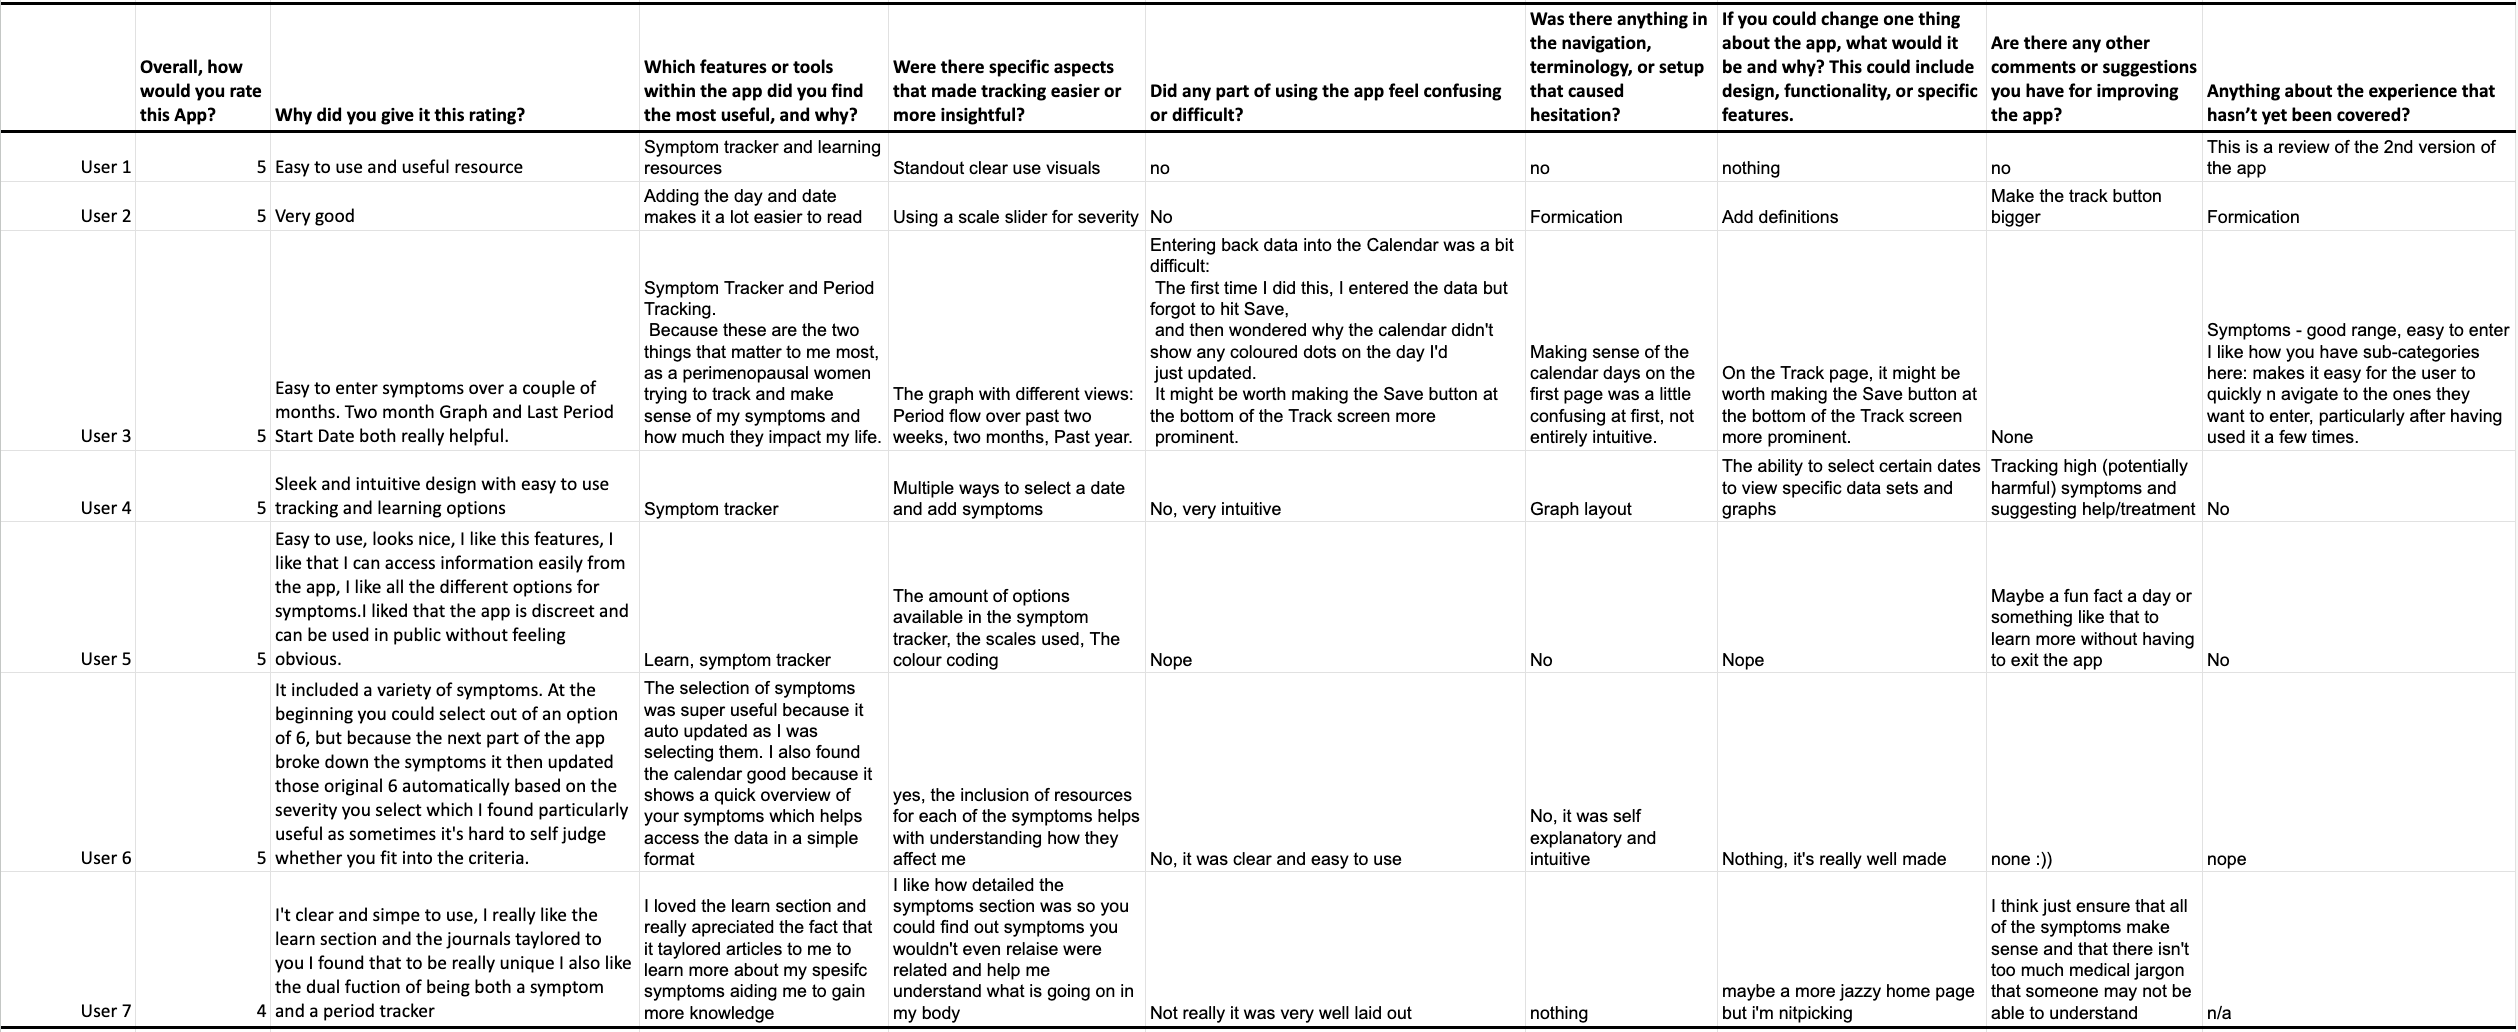
\includegraphics[scale=0.35]{GB-frq.png}
          \caption{Group B Free Response Questions Feedback}
          \label{figure:gb-frq}
        \end{center}
      \end{figure}
    

\subsubsection{MARS Evaluation}
The app was then rated according to the MARS rating system and compared to the other app rated at the beginning of the study. **Results here** 

\subsection{Results of Evaluation}
This Section includes a direct interpretation of the gathered data and evaluation processes. 

\subsubsection{User Requirements Results} 

\subsubsection{Round 1: Web App Evaluation}
The results mean...

percentile of 73 means in top 50\% of all apps as 68 is the middle

\subsubsection{Round 2: React Native Evaluation with Group A}
82nd percentile, significant increase from web app demo video results 

\subsubsection{Round 3: React Native Evaluation with Group B}
92nd percentile, significant increase from group A results.
The changes made to the app were well received by the participants, and the feedback was overwhelmingly positive. The participants found the app easy to use and appreciated the changes made to the look and feel of the app. The average SUS score of 92.5 indicates that the app is highly usable and meets the needs of the target audience.
